\documentclass{beamer}

\usepackage[labelformat=empty]{caption}

\mode<presentation>
{
  \usetheme{Berkeley}
  \usecolortheme{seagull}
  \setbeamercovered{transparent}
}

\title{Nuclear Engineering}
\author{Jeffrey Seifried}
\institute{Ad Delivery Team, Yelp}
\date{Advanced Learning Group, \texttt{2015-03-16}}

\AtBeginSubsection[]
{
  \begin{frame}<beamer>{Outline}
    \tableofcontents[currentsection,currentsubsection]
  \end{frame}
}


\begin{document}

\begin{frame}
  \titlepage
\end{frame}

\begin{frame}{Outline}
  \tableofcontents
\end{frame}


\section{About Me}

    \begin{frame}{I've studied Nuclear Engineering for over a decade}{...and all I got was this stupid tshirt}

        \begin{itemize}

            \item BS at University of Maryland, College Park
            \begin{itemize}
                \item Became a nuclear reactor operator
            \end{itemize}

            \pause

            \item PhD at UC, Berkeley and Lawrence Livermore Lab
            \begin{itemize}
                \item Developed reactor simulations
                \item Propagated uncertainties through them
                \item Helped design a hybrid fusion-fission reactor
            \end{itemize}

            \pause

            \item postdoc
            \begin{itemize}
                \item Developed reactor simulations
                \item Taught a course on nuclear reactor physics
                \item Helped design a thorium-fueled breed and burn reactor
            \end{itemize}
        \end{itemize}

    \end{frame}

\section{Nuclear Energy}

\subsection{The state of the neutron}

    \begin{frame}{Nuclear energy is important right now}

        \begin{columns}[T]

            \begin{column}{0.5\textwidth}
                \begin{figure}
                    \centering
                    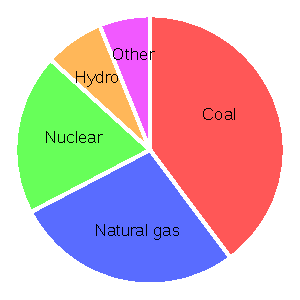
\includegraphics{./img/sources.pdf} \\
                    \caption*{US elecriticity sources (2014)}
                \end{figure}
            \end{column}

            \begin{column}{0.5\textwidth}
                \begin{itemize}
                    \item Fossil Fuels generate 66\%
                    \pause
                    \item Nuclear power generates 20\%
                    \pause
                    \item ...and 60\% of carbon-free electricity
                    \pause
                    \item The most recent plant was built in 1996
                    \pause
                    \item ...its construction began in 1978
                    \pause
                    \item Renewables are ``other''
                \end{itemize}
            \end{column}

        \end{columns}

    \end{frame}

    \begin{frame}{...and soon will be even more important!}

        \begin{itemize}

            \item Coal causes 10 thousand deaths annually in the US
            \pause
            \item One quarter of California air pollution is from China
            \pause
            \item Climate change is just getting ramped up
            \pause

            \vspace{2em}

            \item Global energy use will increase by a third by 2040
            \pause
            \item Natural gas and oil just got a lot cheaper
            \pause
            \item Coal is and always will be cheap

        \end{itemize}

    \end{frame}

\subsection{We've come a long way since 1978}

    \begin{frame}{Light water reactor (LWR) fuel assembly and core}
        \begin{columns}[T]

            \begin{column}{0.5\textwidth}
                \begin{figure}
                    \centering
                    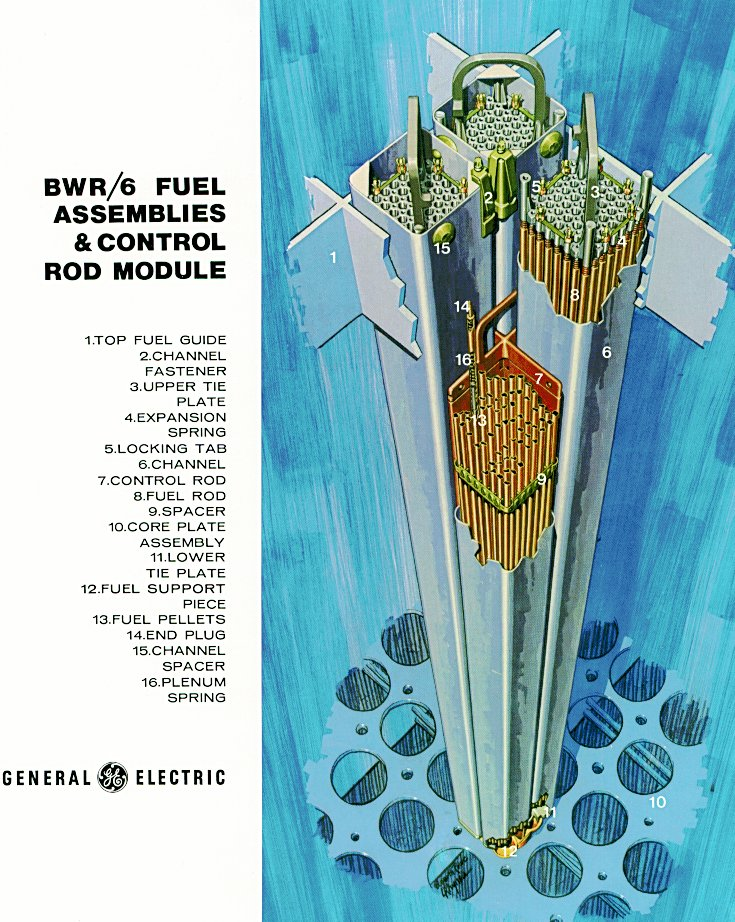
\includegraphics[width=12em]{./img/bwrFuel.png} \\
                    \caption*{}
                \end{figure}
            \end{column}

            \begin{column}{0.5\textwidth}
                \begin{figure}
                    \centering
                    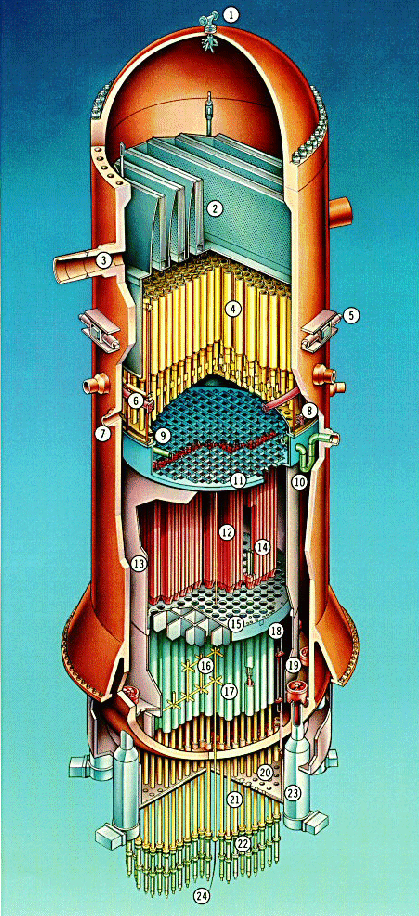
\includegraphics[width=8em]{./img/bwrCore.png} \\
                    \caption*{}
                \end{figure}
            \end{column}

        \end{columns}

    \end{frame}

    \begin{frame}{Boiling Water Reactor (BWR) balance of plant}
        \begin{figure}
            \centering
            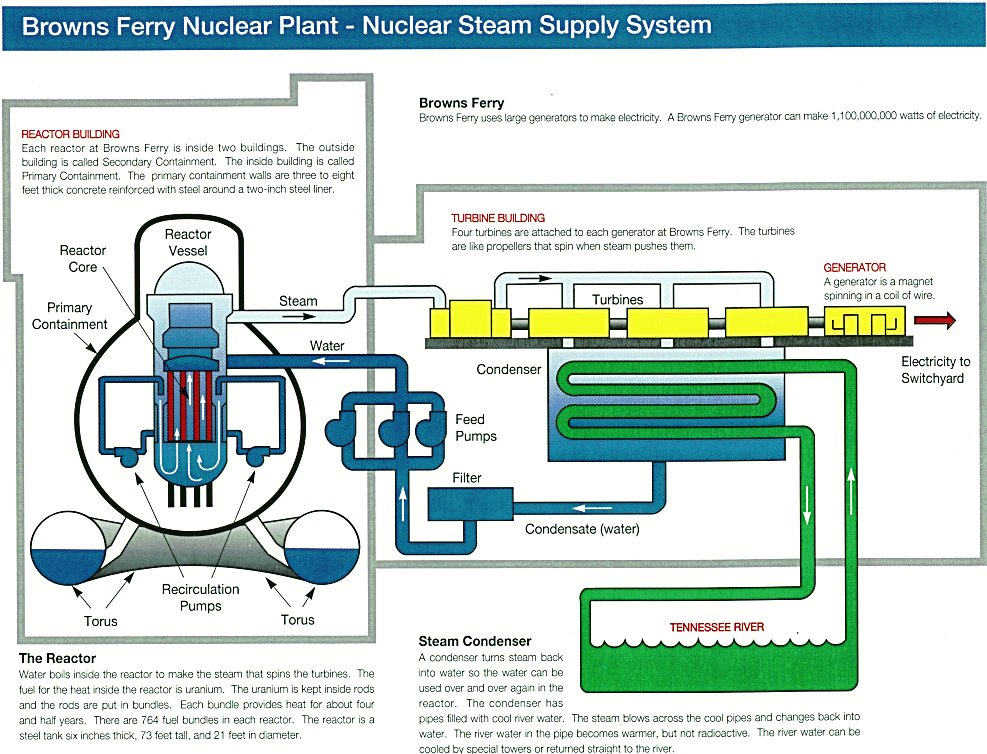
\includegraphics[width=24em]{./img/bwrBop.png} \\
            \caption*{}
        \end{figure}
    \end{frame}

    \begin{frame}{Pressurized Water Reactor (PWR) balance of plant}
        \begin{figure}
            \centering
            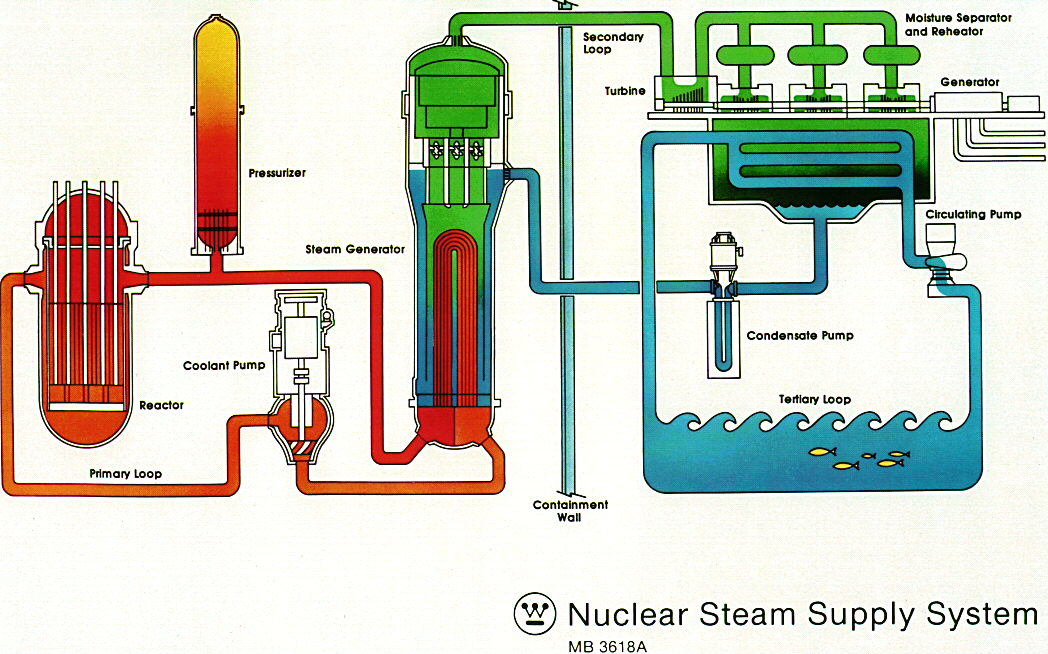
\includegraphics[width=24em]{./img/pwrBop.png} \\
            \caption*{}
        \end{figure}
    \end{frame}

    \begin{frame}{Fast reactors}
    \end{frame}

    \begin{frame}{Breed and burn reactors}
    \end{frame}

    \begin{frame}{Fluoride-salt-cooled high-temperature reactors}
    \end{frame}

    \begin{frame}{Hybrid fusion-fission reactors}
    \end{frame}

\section{Simulations}

\subsection{Solving the neutron transport equation}

    \begin{frame}{Neutrons can be described as existing in a 7-dimensional neutron phase space}
        \begin{figure}
            \centering
            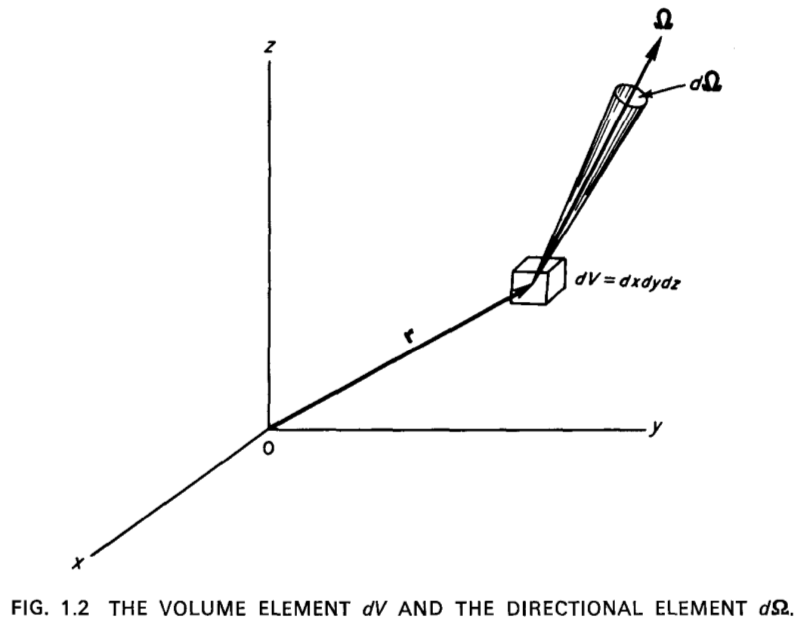
\includegraphics[width=24em]{./img/phaseSpace.png}
        \end{figure}
    \end{frame}

    \begin{frame}{The neutron transport equation balances sources and sinks within this neutron phase space}
        \begin{equation*}
            \begin{split}
                \vec \Omega \cdot \vec \bigtriangledown \; \; \psi(\vec r, E, \vec \Omega) \\
                + \Sigma_{total}(\vec r, E) \; \; \psi(\vec r, E, \vec\Omega) \\
                = \int_0^\infty \! \! \! \! dE \int_{4\pi} \! \! \! \! d\vec\Omega \; \; \Sigma_{scatter}(\vec r, E^\prime \rightarrow E, \vec \Omega^\prime \cdot \vec \Omega) \; \; \psi(\vec r, E^\prime, \vec\Omega^\prime) \\
                + \frac{\chi(E)}{4\pi} \int_0^\infty \! \! \! \! dE^{\prime\prime} \; \; \nu (E^{\prime\prime}) \; \; \Sigma_{fission}(\vec r, E^{\prime\prime}) \; \; \psi(\vec r, E^{\prime\prime}, \vec\Omega^{\prime\prime}) \\
                + \mathcal{S}_{ext}(\vec r, E, \vec\Omega)
            \end{split}
        \end{equation*}
    \end{frame}

    \begin{frame}{Nuclear reaction cross-sections are complicated}
    \end{frame}

\subsection{Solving the Bateman equations}

    \begin{frame}{The Bateman equations describe the time-evolution of isotopes during decay and irradiation}
        \begin{equation*}
            \begin{split}
                \frac{\partial N_i(\vec r, t)}{\partial t} \\
                + \lambda_i \; \; N_i(\vec r, t) \\
                + \int_0^\infty \! \! \! \! dE \; \; \sigma_{absorption,i} ( \vec r, E, \vec\Omega) \; \; \psi(\vec r, E, \vec \Omega) \; \; N_i(\vec r, t) \\
                = \sum_j \left[ b_{j \rightarrow i} \; \; \lambda_j \; \; N_j(\vec r, t) \right] \\
                + \sum_k \left[ b_{k \rightarrow i} \int_0^\infty \! \! \! \! dE \; \; \sigma_{absorption,k} ( \vec r, E, \vec\Omega) \; \; \psi(\vec r, E, \vec \Omega) \; \; N_k(\vec r, t) \right] \\
            \end{split}
        \end{equation*}
    \end{frame}

\section*{Summary}

    \begin{frame}{Summary}
    \end{frame}

\end{document}
